\documentclass[a4paper,11pt]{article}

\usepackage{array}
\usepackage{graphicx}
\usepackage[latin9]{inputenc}
\usepackage[german]{babel}
\usepackage[T1]{fontenc}
\usepackage[left=3cm,right=2cm]{geometry}
\usepackage[colorlinks=false, pdfborder={0 0 0}]{hyperref}	%Links im Inhaltsverzeichniss
\usepackage{pdflscape}
\usepackage{here} % hiermit k�nnen die Bilder dort platziert werden, wo man sie haben m�chte!!! Verwendung: \begin{figure}[H]...\end{figure}

\begin{document}
\newpage

\title{Thema der Arbeit}
\author{
Christof Ochmann\\ Matrikelnummer: 35989 \\Hochschule Zittau/G�rlitz\\ Fakult�t Elektrotechnik und Informatik\\ IIm11
\and
Stefan L�ttke \\ Matrikelnummer: xxxxx \\Hochschule Zittau/G�rlitz\\ Fakult�t Elektrotechnik und Informatik\\ IIm11
\and
Ingo K�rner \\ Matrikelnummer: 40586 \\Hochschule Zittau/G�rlitz\\ Fakult�t Elektrotechnik und Informatik\\ IIm11
}
\date{2012-02-02}

\maketitle
\newpage

\tableofcontents
\newpage

\part{Wohnheimprojekt}

\part{Performance-Messungen von Datenbank Konfigurationen}

\section{Theorie}
\section{Einleitung}\label{einleitung}
Ziel dieses Projektes ist die Performance eines relationalen Datenbankmagagementsystems f�r bestimmte Konfigurationen zu testen. Die Konfiguration ergibt sich aus den Anforderungen, die an das DBMS bzw. die konkrete Datenbank gestellt werden. 
Es ergibt sich die Frage, f�r welche konkrete Anforderung welche konkrete Konfiguration gew�hlt werden sollte? Um diese Frage zu beantworten, sind mehrere Schritte n�tig. Es wird zuerst ein DBMS exemplarisch ausgew�hlt. Dann wird f�r dieses DBMS ein ERD angefertigt, dass die Tabellen beschreibt. Um die Performance zu testen, muss ein Datengenerator geschrieben werden, der die Testdaten f�r die Tabellen generiert. Die konkreten Anforderungen, die an den Datengenerator gestellt werden, m�ssen analysiert werden. Dann wird der Generator entworfen, implementiert und getestet. F�r den Datengenerator wird ein Build Mangagement Tool eingesetzt sowie Frameworks f�r Dependency Injection und zum Testen der Anwendung. Dann werden f�r die Konfigurationen Queries auf den mit Testdaten bef�llten Tabellen gefahren und die Antwortzeiten gemessen. Die Messungen erfolgen alle auf einem Referenzsystem. So k�nnen verschiedene Konfigurationen �ber ihre Performancewerte miteinander verglichen werden.
\section{Aufgabenstellung}\label{Aufgabenstellung}
In diesem Projekt soll die Abfrage-Performace f�r ein bestimmtes Szenario gemessen werden. Dazu ist ein Szenario auszuw�hlen, das im Bereich OLAP und Data Warehouse angesiedelt ist. F�r das Szenario sind geeignete Konfigurationen zu w�hlen. Konfigurationen unterscheiden sich in Art- und Anzahl von Indexen und in den Partitionierungsarten. Es wird angenommen, dass jede Konfiguration f�r eine bestimmte Art von Abfragen besonders geeignet ist. Es sollen verschiedenartige Abfragen gew�hlt werden, f�r die jeweils die Performance gemessen wird. Um die Performance messen zu k�nnen, ist ein ERD f�r ein gew�hltes Szenario anzufertigen. Die Tabellen des ERD sollen mit Testdaten gef�llt werden. Dazu ist ein Datengenerator anzufertigen. Die Abfragen werden auf die gef�llten Tabellen angewendet. Die Zeit, die ein Query braucht, um auf einer bestimmten Konfiguration ausgef�hrt zu werden, wird gemessen. Das Messergebnis wird mit der Annahme verglichen und ausgewertet.
\subsection{EasyMock}
EasyMock 3.0 ist ein Test-Framework zur dynamischen Generierung von Mock Objekten f�r Schnittstellen und Klassen. Mock-Objekte werden f�r Unit-Tests von Java-Programmen verwendet.

\subsubsection{Was ist ein Mock-Objekt?}
Beim Unit-Testing kollaborieren Units mit anderen Units. Die Kollaborateure werden durch Mock Objekte simuliert. Im Gegensatz zu einem Stub �berpr�ft das Mock-Objekt, ob es wie erwartet verwendet wurde. In einem Unit-Test werden Klassen bzw. Methoden isoliert von ihrer Umgebung getestet. Um die Testobjekte isoliert zu testen, m�ssen die Schnittstellen des Testobjekts durch Mock-Objekte ersetzt werden. Die Mock-Objekte sind Platzhalter f�r die echten Objekte. Das Verhalten eines dynamischen Mock-Objekts wird nicht in einer Klasse programmiert, sondern von dem Unit-Test aufgezeichnet. Es m�ssen keine Klassen von Hand geschrieben werden. Es muss auch kein Quellcode der Mock-Klassen, mit den echten Klassen synchron gehalten werden. Mock-Objekte werden bei EasyMock ''on the fly'' generiert, sind sicherer gegen Refactoring und damit besonders f�r Test Driven Development geeignet.

\subsubsection{Wie wird EasyMock benutzt?}
Um EasyMock zu benutzen, sind folgende Schritte n�tig:
\begin{enumerate}
	\item das Mock-Objekt von der Klasse / Schnittstelle die simuliert werden soll, erzeugen und dem zu testenden Objekt �bergeben,
	\item das erwartete Verhalten aufzeichnen,
	\item das Mock-Objekt auf Wiedergabe-Modus stellen,
	\item verifizieren, ob das Mock-Objekt auch so benutzt wurde, wie in Schritt zwei spezifiziert
\end{enumerate}
\section{Datengenerator}
Die Testdaten zum F�llen der Tabellen werden mit einem Datengenerator erzeugt.

\subsection{Analyse}
Der Datengenerator soll die Testdaten f�r die vier Tabellen 
\begin{itemize}
	\item Kunde,
	\item Produkt,
	\item Warenkorb,
	\item WarenkorbProdukt
\end{itemize}
erzeugen und in die Tabellen schreiben. Dabei sollen dem Generator vier Parameter beim Start �bergeben werden:
\begin{enumerate}
	\item die Anzahl der zu erzeugenden Kunden
	\item die Anzahl der zu erzeugenden Produkte
	\item die Anzahl der Warenk�rbe pro Kunde
	\item die Anzahl der Produkte im Warenkorb
\end{enumerate}

Der Generator muss f�r alle beliebigen Startparameter die Tupel der einzelnen Tabellen korrekt miteinander verkn�pfen. Deswegen erzeugt der Generator auch die Prim�r- und Fremdschl�ssel der Tupel selbst. 
Die maximale Anzahl der Warenk�rbe ergibt sich aus der Anzahl der Kunden * der Anzahl der Warenk�rbe pro Kunde. In der Warenkorbtabelle m�ssen bei einer Anzahl von z.B. 10 Warenk�rben pro Kunde auch je 10 Warenk�rbe existieren, die mit ihrem Fremdschl�ssel auf den jeweiligen Kunden zeigen. In der Warenkorbtabelle sollen im Datum alle Monate des Jahres 2011 gleichm��ig verteilt vorkommen. 

Die maximale Anzahl der Bestellzeilen ergibt sich aus der Anzahl der Kunden * der Anzahl der Warenk�rbe pro Kunde * der Anzahl der Produkte in einem Warenkorb. Die m�glichen Produkte sollen gleichm��ig �ber alle Bestellzeilen verteilt sein. In der WarenkorbProdukt-Tabelle m�ssen bei einer Anzahl von z.B. 7 Produkten im Warenkorb auch je 7 Bestellzeilen existieren, die mit ihrem Fremdschl�ssel auf den jeweiligen Warenkorb zeigen.

F�r jede Tabelle soll ausgegeben werden, wieviel Zeit der Generator insgesamt f�r den Schreibvorgang ben�tigte. Damit wird es auch m�glich, die Schreibperformance einer Datenbankkonfiguration zu messen und auszuwerten.

\subsubsection{Anwendungsfalldiagramm}

Die Abbildung \ref{fig:AnwendungsfalldiagrammDatengenerator} auf Seite \pageref{fig:AnwendungsfalldiagrammDatengenerator} zeigt das Anwendungsfalldiagramm des Prototypen.

\subsubsection{User Stories}

1. AF - Datengenerator mit Aufrufparametern ausf�hren
Um die Testdaten zu generieren und in die Tabellen zu schreiben ruft der Anwender den Datengenerator als Jar-Datei �ber die Kommandozeile auf und �bergibt ihm die folgenden vier Aufrufparameter in gegebeneer Reihenfolge:
\begin{enumerate}
	\item die Anzahl der zu erzeugenden Kunden
	\item die Anzahl der zu erzeugenden Produkte
	\item die Anzahl der Warenk�rbe pro Kunde
	\item die Anzahl der Produkte im Warenkorb
\end{enumerate}

2. AF - Zeiten f�r die Schreibvorg�nge �bernehmen
Der Anwender notiert sich die vom Generator auf der Konsole ausgegebenen Gesamtzeiten der einzelnen Schreibvorg�nge.

3. AF - Anzahl der insgesamt geschriebenen Tupel pro Tabelle �bernehmen
Der Anwender notiert sich die auf der Konsole ausgegebenen Werte der vom Generator insgesamt geschriebenen Tupel f�r jede Tabelle.

Die Abbildung \ref{fig:AnalyseDatengenerator} auf Seite \pageref{fig:AnalyseDatengenerator} zeigt das Analyseklassendiagramm des Datengenerators.

\subsubsection{UI-Mockup}
Die Abbildung \ref{fig:UI-MockUp} auf Seite \pageref{fig:UI-MockUp} zeigt das UI-Mockup des Datengenerators.



\begin{figure}[htp]
\centering
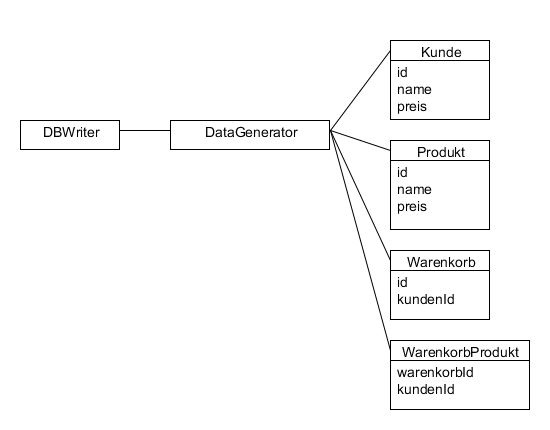
\includegraphics[width=0.8\textwidth]{Ingo/Bilder/AnalyseDatengenerator.png}
\caption{Analyse Datengenerator}
\label{fig:AnalyseDatengenerator}
\end{figure}

\begin{figure}[htp]
\centering
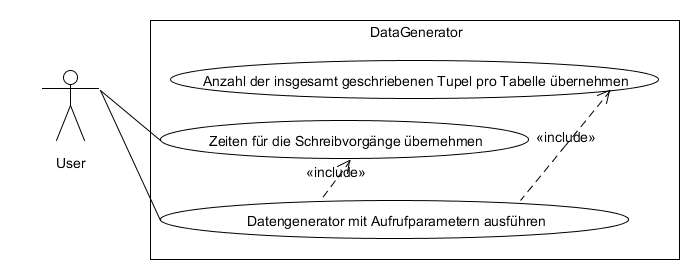
\includegraphics[width=0.8\textwidth]{Ingo/Bilder/AnwendungsfalldiagrammDatengenerator.png}
\caption{Anwendungsfalldiagramm Datengenerator}
\label{fig:AnwendungsfalldiagrammDatengenerator}
\end{figure}


\begin{figure}[htp]
\centering
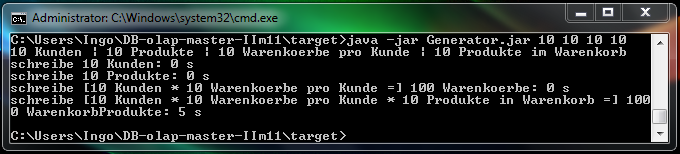
\includegraphics[width=0.8\textwidth]{Ingo/Bilder/UIMockUp.png}
\caption{UI-MockUp}
\label{fig:UI-MockUp}
\end{figure}

\newpage
\begin{flushleft}
\begin{thebibliography}{sotief}
\bibitem{bib1}{\textit{''Buchtitel''} Author}
\bibitem{bib2}{\it \begin{verbatim}http://www.google.de \end{verbatim}} 
\end{thebibliography}
\end{flushleft}




\newpage
\begin{landscape}
\section*{Arbeitsaufteilung}
\begin{table}[h]

	\begin{center}
		\begin{tabular}{|l||c|c|c|c|c|c|}
	  	\hline
	  		 \textbf{Arbeit}		&	\textbf{Cristof Ochmann}	&	\textbf{Stefan L�ttke}	& \textbf{Ingo K�rner}  \\ \hline \hline
				  			Thema 1   	&     x              &                   &                     \\
				  			Thema 2	    &                   &          	x	      & 	             			\\ \hline
							  Thema 3   	&                   &                   &     x 			            \\ 
			  			 \hline
			  			 \hline
					Belegkapitel 		
					
%%%%%%%%%%%%%%%%%%%% Christof					
					&									     
					\ref{Einleitung}, \& \ref{Einleitung}
					
%%%%%%%%%%%%%%%%%%%% Stefan					
					&                       
					~\ref{Einleitung}
%%%%%%%%%%%%%%%%%%%% Ingo					
					&                     
					~\ref{Einleitung}, ~\ref{Einleitung}, ~\ref{Einleitung} - ~\ref{Einleitung}
					\\\hline\hline			       
		\end{tabular}			
	\end{center}
\end{table}
\end{landscape}


\newpage
\section*{Eigenst�ndigkeitserkl�rung} 

Hiermit erkl�re ich, dass ich diese Arbeit selbst�ndig verfasst habe.\\
Mir ist bekannt, dass jede Form des Plagiats mit der Note 5 (Betrugsversuch) bewertet wird. \\

\textbf{Ochmann, Christof} \\ 
\renewcommand{\baselinestretch}{1.25}\normalsize{
\noindent\hspace*{80mm}%
Unterschrift:\\}

\textbf{L�ttke, Stefan}\\
\renewcommand{\baselinestretch}{1.25}\normalsize{
\noindent\hspace*{80mm}%
Unterschrift:\\}

\textbf{K�rner, Ingo}\\
\renewcommand{\baselinestretch}{1.25}\normalsize{
\noindent\hspace*{80mm}%
Unterschrift:\\}

\end{document}
